\section{Study of systematics in ringdown measurements in real, non-Gaussian noise}\label{sec:noise_systematics}


Inferences of all parameters in this paper have been done under the
assumption that the noise in the detectors is stationary and
Gaussian. In other words, detector noise follows a normal distrubution
with zero mean and a PSD, $S_n(f)$, that is not a function of time, at
least during the internal of the GW signal. This
allows us to write the Bayesian likelihood function in the form given
in Eqs.~(\ref{eq:likelihood}) and ~(\ref{eq:nwip}), and perform all the
parameter estimation that follows in the results sections. However,,
LIGO-Virgo noise can often have features that deviate from
stationarity and Gaussianity. If such features are not taken into
account appropriately, final estimates of parameters can get
biased. Here we demonstrate one such case by injecting in real noise a
GW190521-like signal and showing how parameter estimates can be biased
\ab{when} our \sout{understanding} \ab{description} of detector noise is not complete.

%%%%%%%%%%%%%%%%%%%%%%%%%%%%%%%%%%%%%%%%%%%%%%%%%%%%%%%%%%%%%%%
%%%%%%%%%%%%%%%%%%%%%%%%%%%%%%%%%%%%%%%%%%%%%%%%%%%%%%%%%%%%%%%
\begin{figure}
\begin{center}
        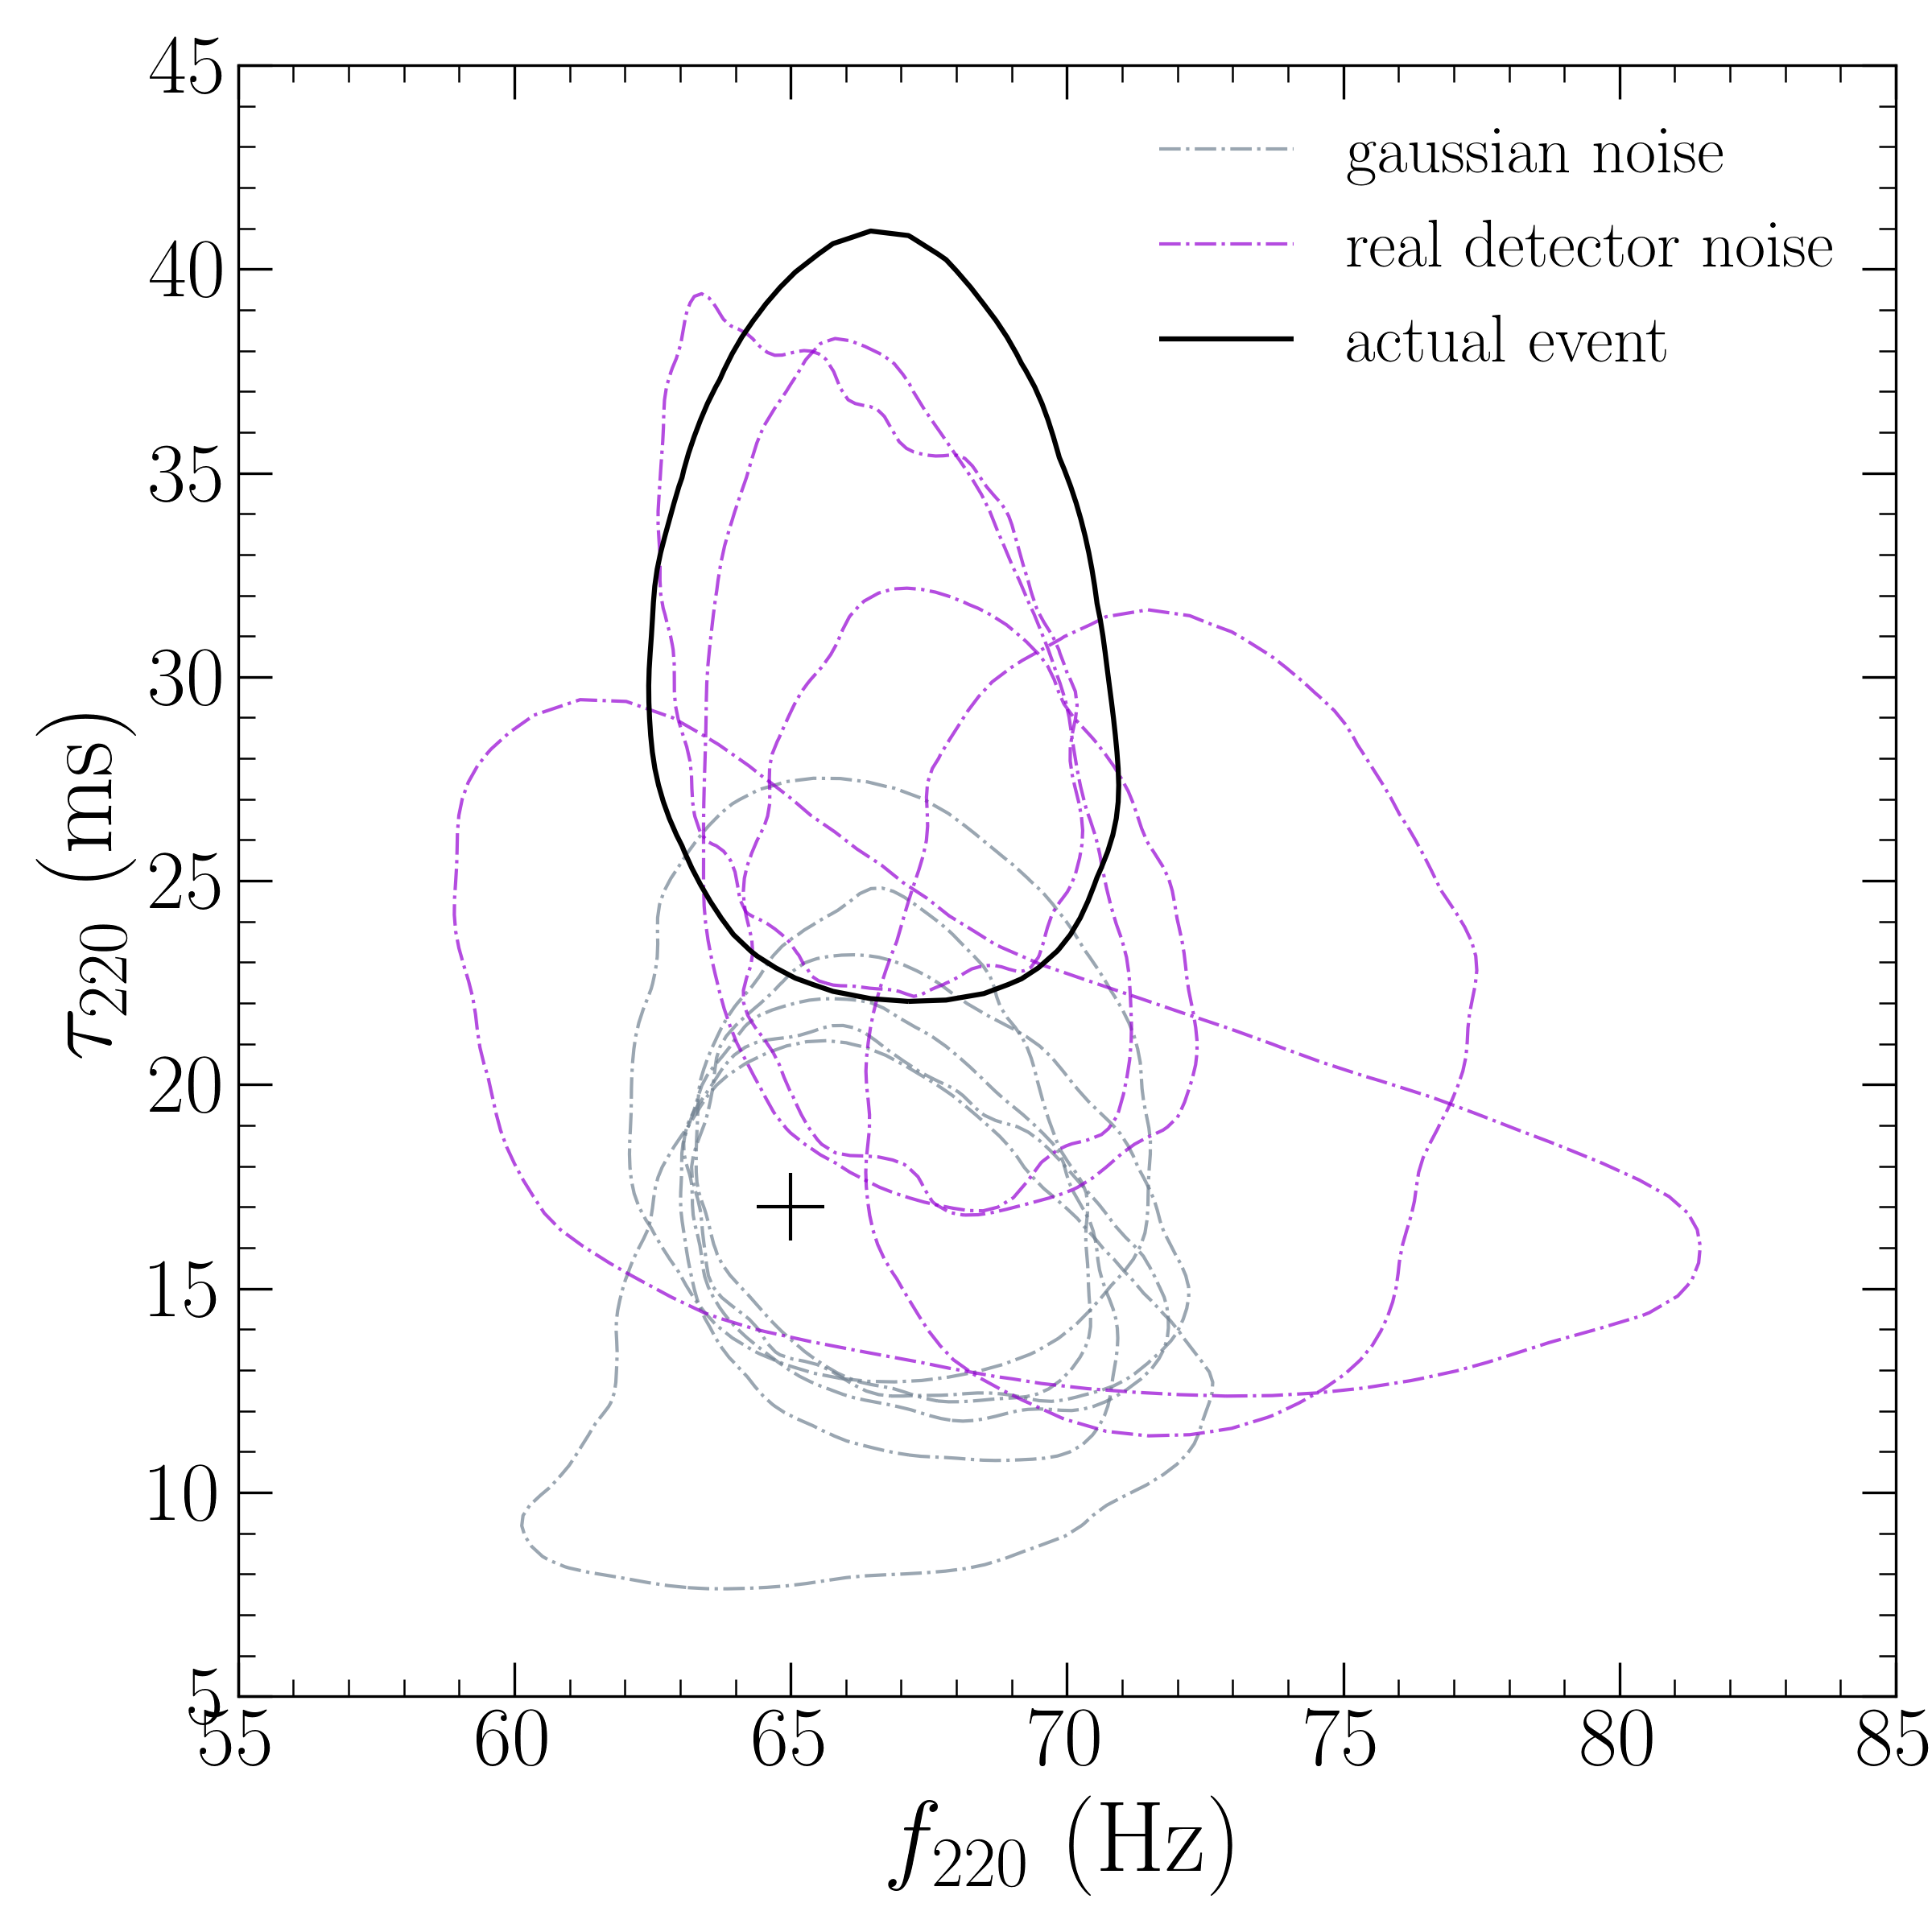
\includegraphics[width=0.4\textwidth]{figures/S190521g_swinjs.png}
        \caption{\textcolor{red}{FINAL RESULT} 90 \% credible level on the posterior probability distribution of the frequency and damping time of $(2,\pm 2)$ mode, $(\fgr{220}, \taugr{220})$ using synthetic \texttt{NRSur} signals with parameters similar to the GW event, GW190521, in Gaussian noise (grey dot-dashed lines) and real interferometric noise (green dot dashed lines). The GR prediction for the frequency and damping time is indicated by the black cross. While the Gaussian noise simulations are consistent with the prediction, at least 3 or the 5 real noise simulation are not. The black curve corresponds to the measurements of the real event GW190521 reported in Ref.~\cite{Abbott:2020jks}. All signals are recovered using the $\pSEOB$ model.}
        \label{fig:21g_systematics}
\end{center}
\end{figure}
%%%%%%%%%%%%%%%%%%%%%%%%%%%%%%%%%%%%%%%%%%%%%%%%%%%%%%%%%%%%%%%
%%%%%%%%%%%%%%%%%%%%%%%%%%%%%%%%%%%%%%%%%%%%%%%%%%%%%%%%%%%%%%%

We choose a spin, precessing NR-surrogate model \ab{\texttt{NRSur}~\footnote{This waveform model is 
called \texttt{NRSur7dq4} in LAL.}} (valid up to mass ratio 4) to simulate the actual GW190521 signal
observed by the LIGO and Virgo detectors~\cite{Abbott:2020tfl} (see
Table I of Ref.~\cite{Abbott:2020tfl})). The choice of the
\texttt{NRSur} model is motivated by the fact that it is the most
accurate model in the parameter range described by GW190521\ab{, because 
it is built by directly interpolating NR waveforms.} In
Fig.~\ref{fig:21g_systematics}, we indicate with a black cross \comment{AB: I am 
confused, a model doesn't predict one value by a posterior distribution. What do you 
mean?} what
the injected \texttt{NRSur} signal predicts for the QNM $(\ell=2,m=2)$
frequency and damping time. For comparison, we also show with a
black solid curve the results obtained when recovering the actual
signal GW190521 with the $\pSEOB$ model. As seen in the plot,
while the measurement of the frequency is consistent with the
prediction, we overestimate the damping time.

\ab{To understand such offset in the decay time, we proceed as follows.} 
The actual GW190521 event was observed at a GPS time, 1242442967.61
seconds (roughly 03:02:49 UTC, May 21, 2019). We select a time period
of about 2.5 hours around this GPS time\ab{, create synthetic signals 
with the \texttt{NRSur} model and inject them in different stretches
of the real detector noise} around the time of the actual GW event. The
PSDs of GW detectors are expected to vary over longer durations of
time, and hence the 2.5 hour stretch of noise we consider can be
assumed to have noise-properties similar to the time of the actual
event. \ab{Then, we perform Bayesian analysis against those injections 
using the $\pSEOB$ model.} The results are indicated by green curves in
Fig.~\ref{fig:21g_systematics}. As it can be seen from the figure, for
3 of the 5 noise realizations, corresponding to $t_0-1$ hour,
$t_0+0.5$ hours, and $t_0+1$ hour, we recover a damping time similar to
the \ab{one obtained when using the $\pSEOB$ model against the actual event GW190521 
(black curve)}, where $t_0$ is the GPS time of the actual event. For
the other two noise realizations, \ab{the $\pSEOB$ model estimates 
consistently} the damping time, but \ab{has} an off-set frequency, 
while the fifth noise realization is consistent with both predictions.  
\ab{This study suggests} that a bias in the measurements of the damping time 
for the actual event GW190521 can be explained \ab{as due to} an incomplete 
description of the noise at the time of the event.

The reader might question the judiciousness of using an aligned-spin
waveform model, like $\pSEOB$, to measure a signal like GW190521 which
appears to be precessing, especially because an incomplete
understanding of the underlying signal can also lead to biases in
measured quantities, as we have already demonstrated in
Sec.~\ref{ssec:ngr_signal}. In order to explore possible effects of
missing information about in-plane spins in the $\pSEOB$ model, we repeat the
above study of injecting synthetic signals using \texttt{NRSur}
and recovering using the $\pSEOB$ model, \ab{but this time, instead of
using real detector noise, we use Gaussian noise (i.e., realizations
of noise sampled from a predicted detector PSD).} Since the properties
of the noise are completely understood in this case, any residual
measurement biases can be completely attributed to diffferences in the
waveform model. The 2D posterior distributions of the frequency and
damping time measured using these Gaussian-noise signals are shown by
the grey curves in Fig.~\ref{fig:21g_systematics}. We find the
measurements to be completely consistent with the predictions of the
frequency and damping time, thus concluding that a lack of in-plane
spins in the $\pSEOB$ model does not affect our measurements of the
QNM properties. The fact that the measurement of ringdown quantities
are robust against an incomplete description of \ab{the inspiral signal 
is a crucial property of our method.} 

%%%%%%%%%%%%%%%%%%%%%%%%%%%%%%%%%%%%%%%%%%%%%%%%%%%%%%%%%%%%%%%
%%%%%%%%%%%%%%%%%%%%%%%%%%%%%%%%%%%%%%%%%%%%%%%%%%%%%%%%%%%%%%%
\begin{figure*}
\begin{center}
        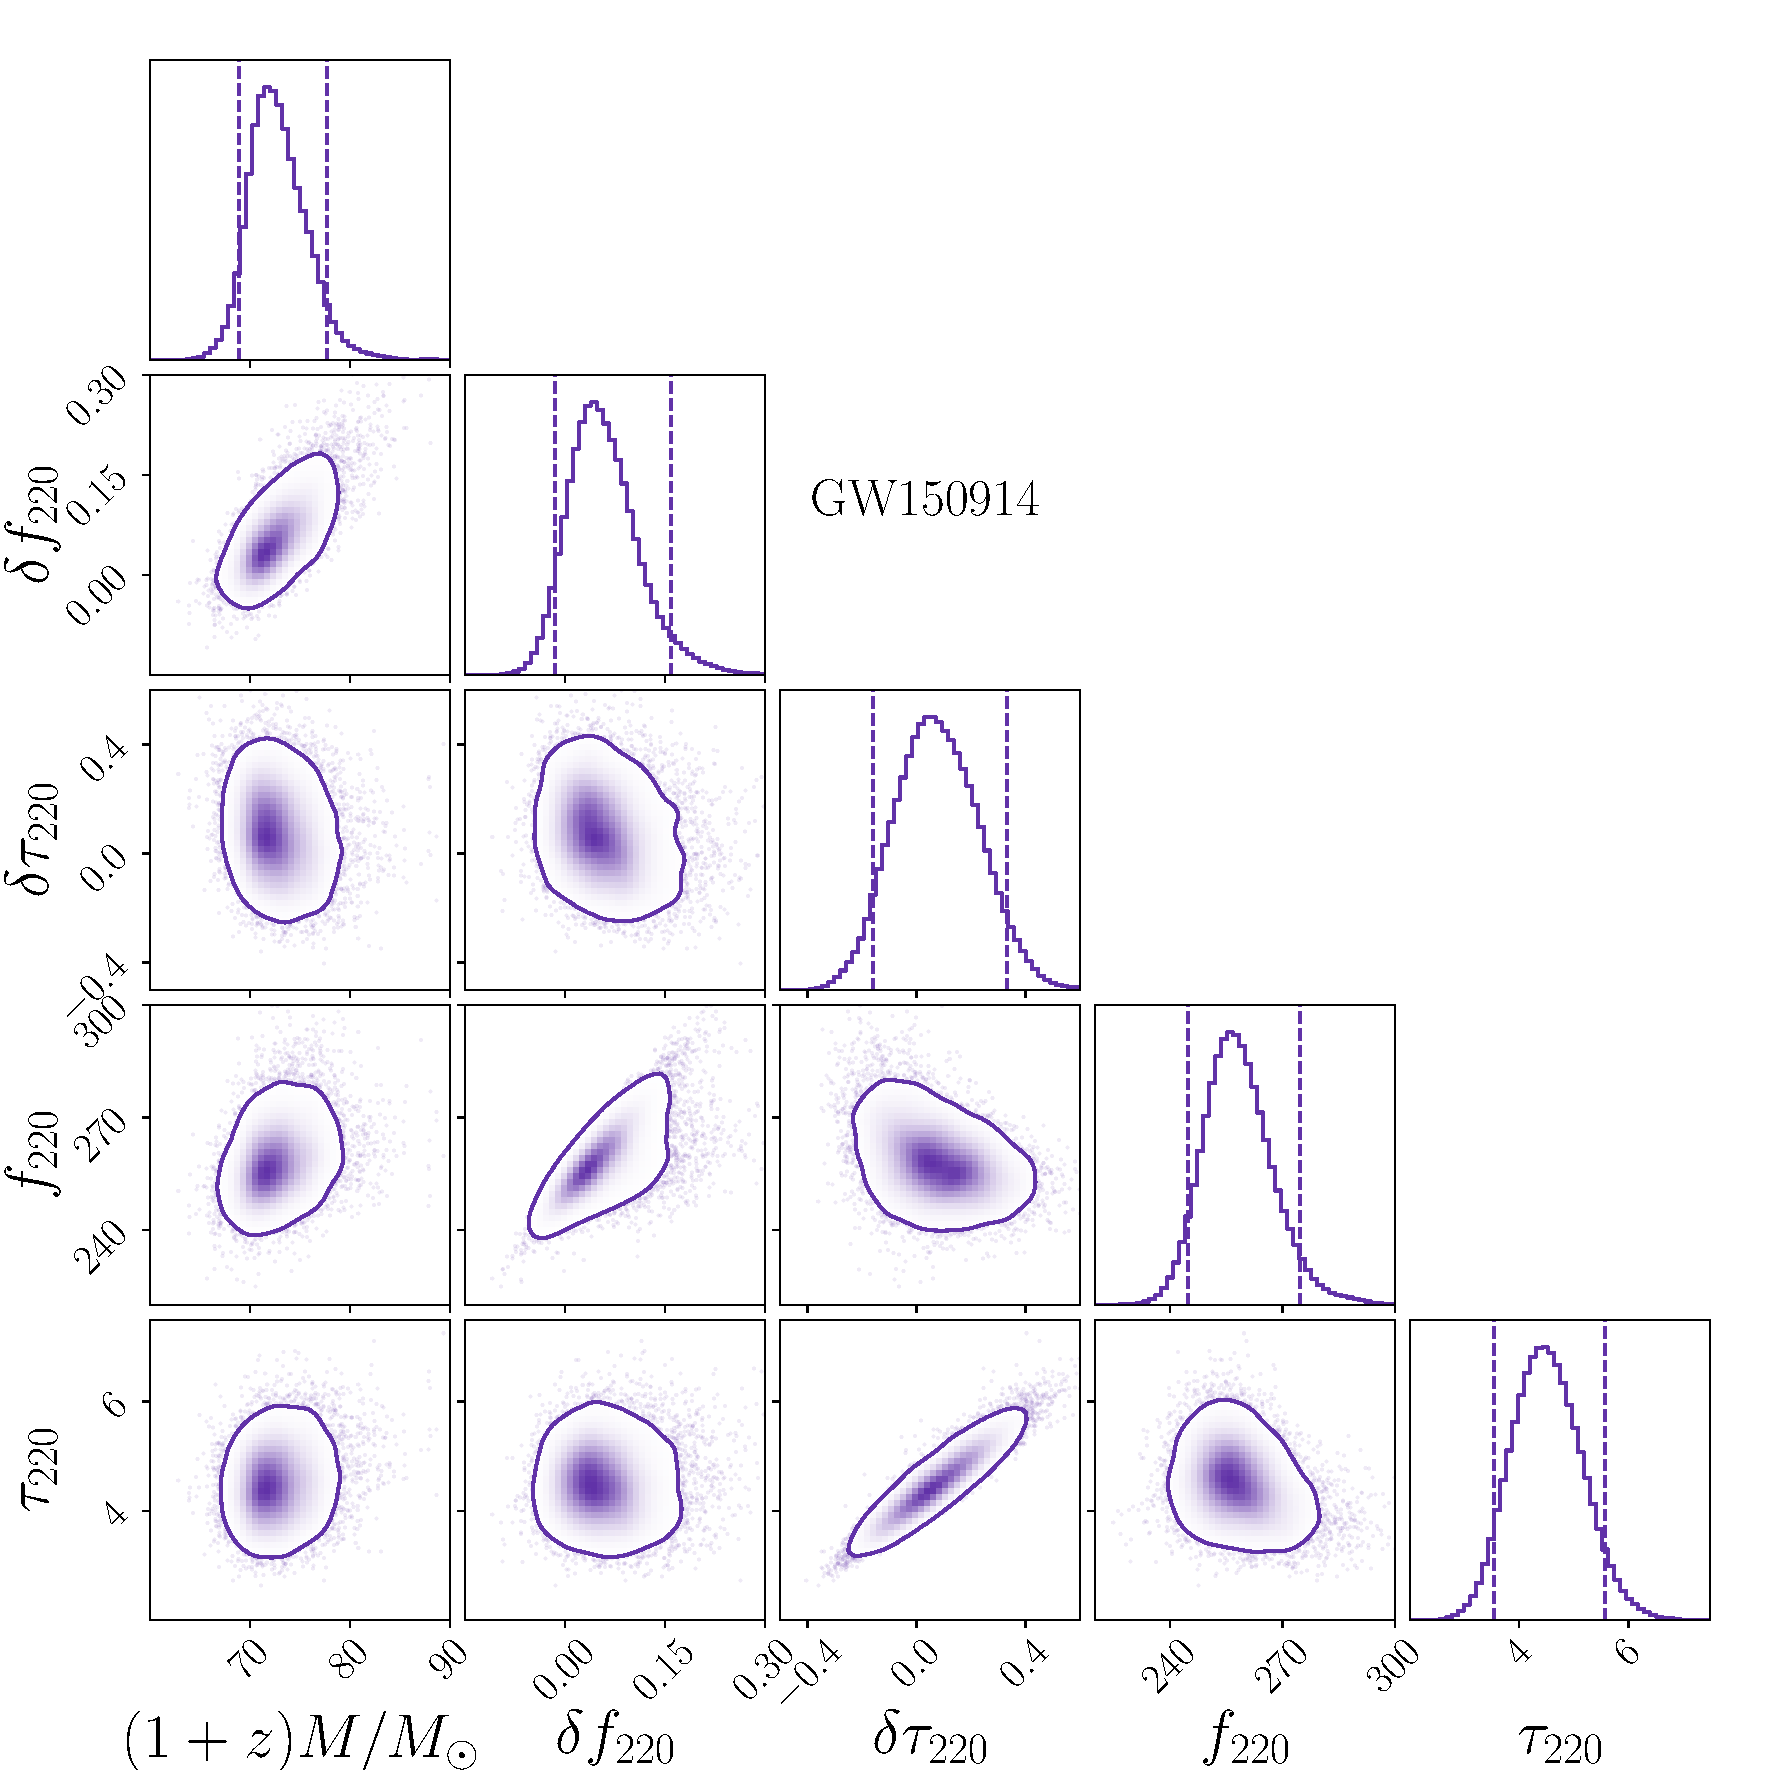
\includegraphics[width=0.45\textwidth]{figures/mtotal_qnm_params_degeneracy_GW150914.pdf}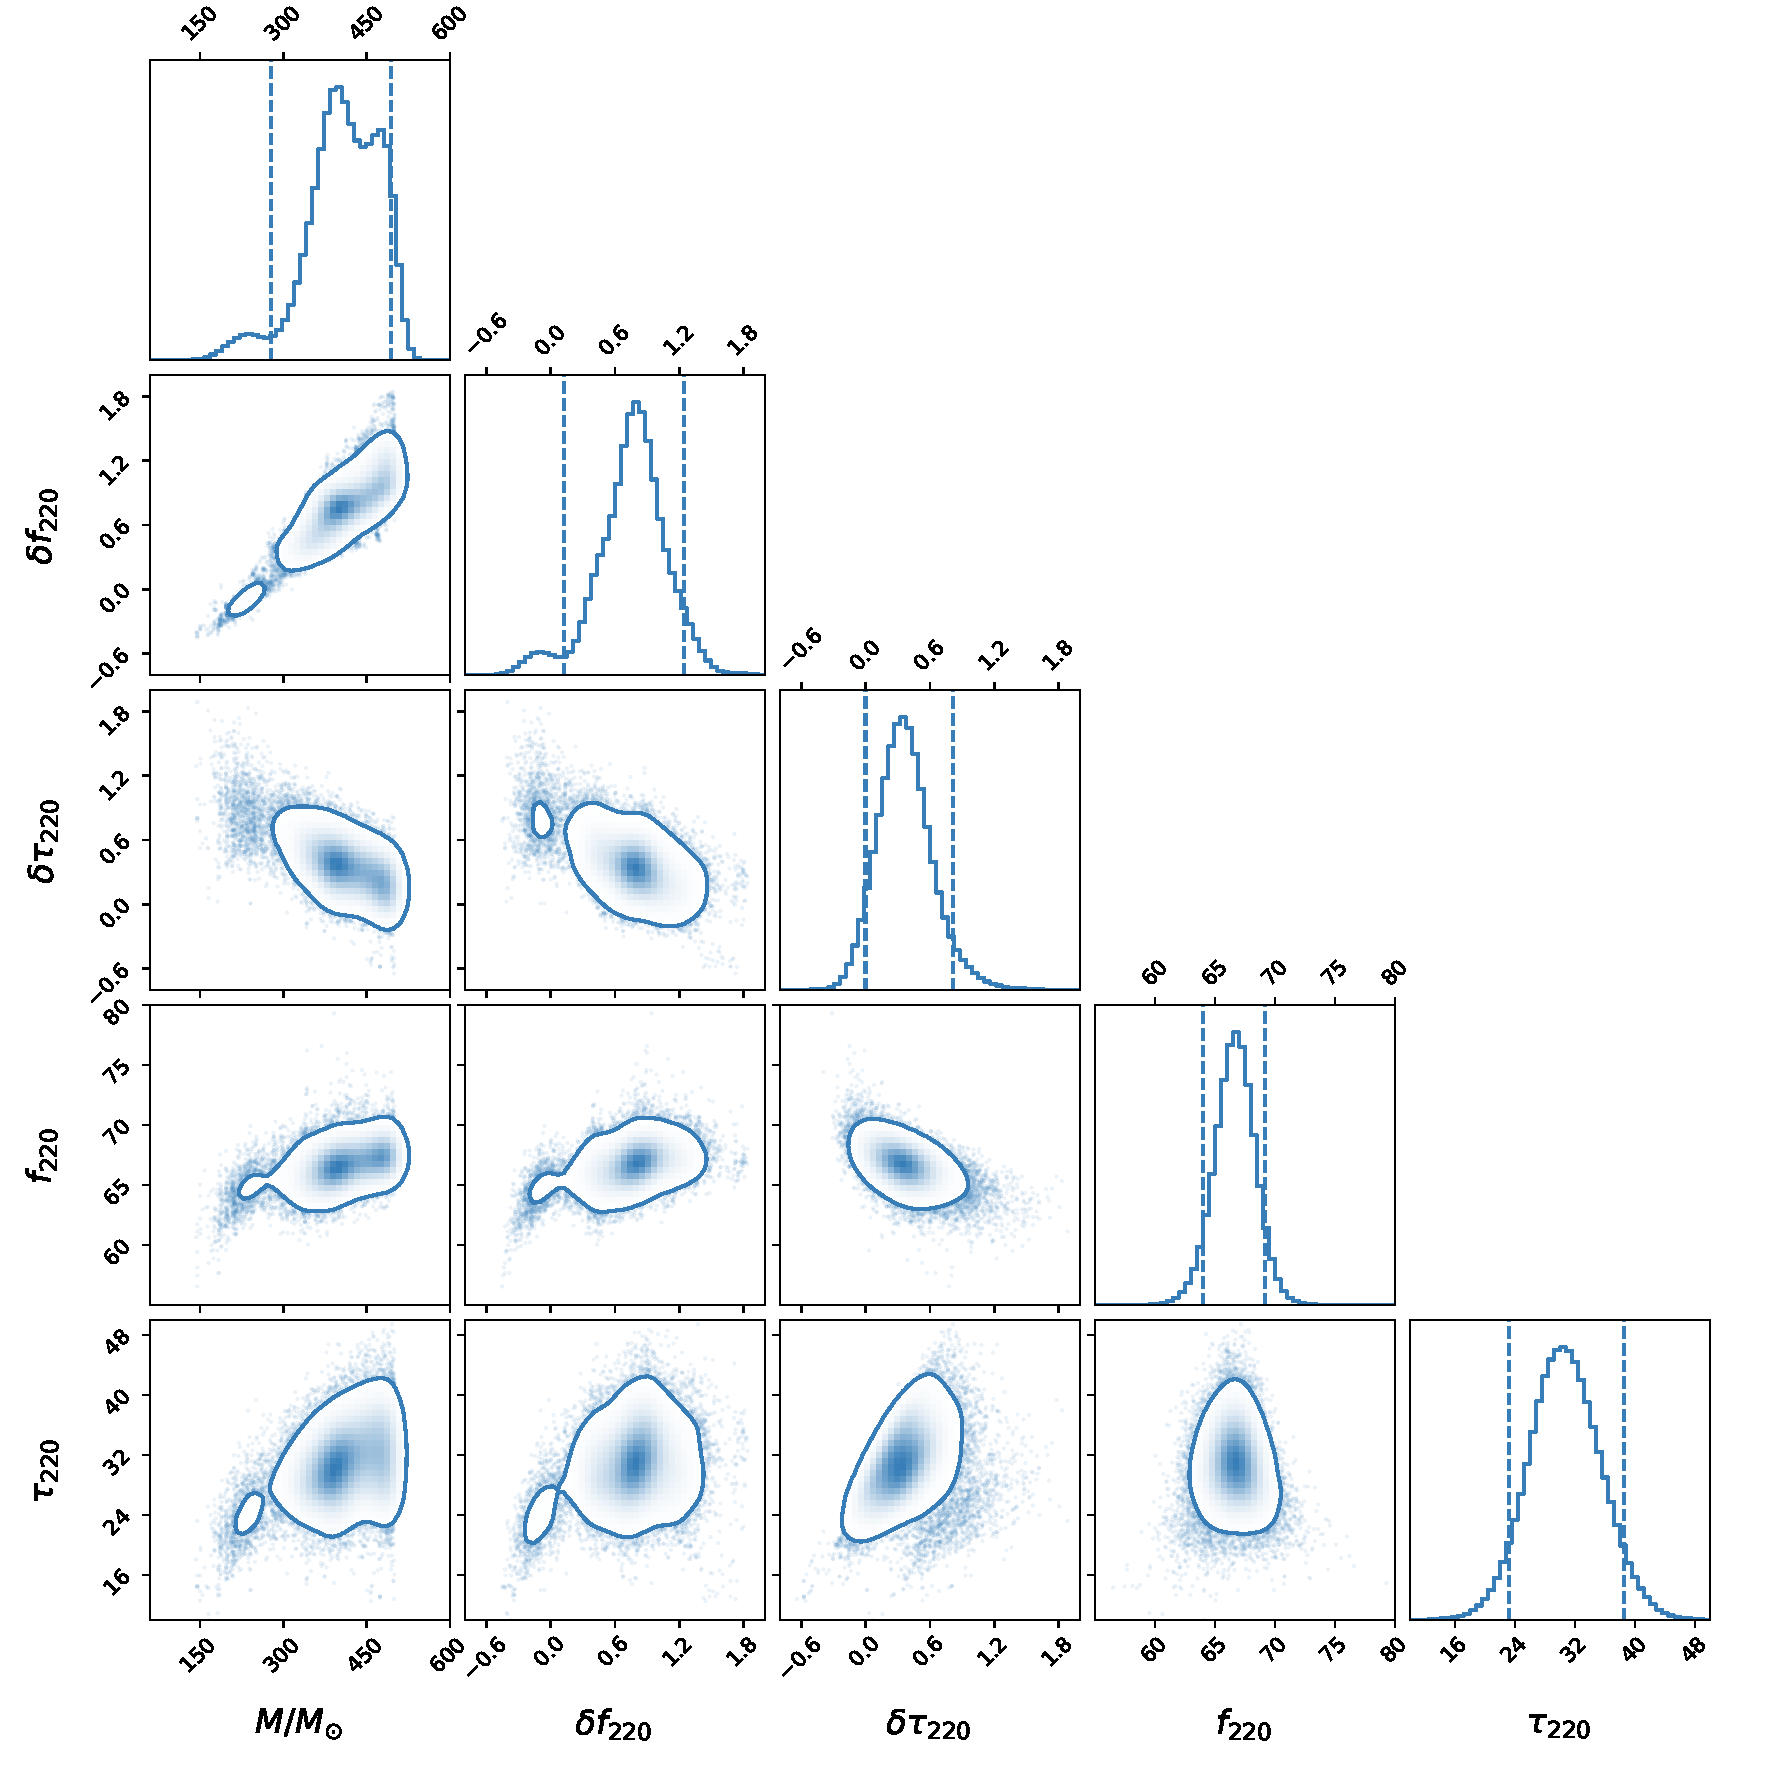
\includegraphics[width=0.45\textwidth]{figures/mtotal_qnm_params_degeneracy_S190521g.pdf}
        \caption{Left panel: GW150914, Right panel: GW190521. Describe the correlations in this caption}
        \label{fig:correlations}
\end{center}
\end{figure*}
%%%%%%%%%%%%%%%%%%%%%%%%%%%%%%%%%%%%%%%%%%%%%%%%%%%%%%%%%%%%%%%
%%%%%%%%%%%%%%%%%%%%%%%%%%%%%%%%%%%%%%%%%%%%%%%%%%%%%%%%%%%%%%%